%%%%%%%%%%%%%%%%%%%%%%%%%%%%%%%%%%%%%%%%%
% A beamer poster style for the University of Oxford. Atilim Gunes Baydin <gunes@robots.ox.ac.uk>, November 2016.
% Based on the I6pd2 style created by Thomas Deselaers an Philippe Dreuw.
%
% Dreuw & Deselaer's Poster
% LaTeX Template
% Version 1.0 (11/04/13)
%
% Created by:
% Philippe Dreuw and Thomas Deselaers
% http://www-i6.informatik.rwth-aachen.de/~dreuw/latexbeamerposter.php
%
% This template has been downloaded from:
% http://www.LaTeXTemplates.com
%
% License:
% CC BY-NC-SA 3.0 (http://creativecommons.org/licenses/by-nc-sa/3.0/)
%
%%%%%%%%%%%%%%%%%%%%%%%%%%%%%%%%%%%%%%%%%

%----------------------------------------------------------------------------------------
%   PACKAGES AND OTHER DOCUMENT CONFIGURATIONS
%----------------------------------------------------------------------------------------

\documentclass[final,hyperref={pdfpagelabels=false}]{beamer}

\usepackage[orientation=portrait,size=a0,scale=1.5]{beamerposter} % Use the beamerposter package for laying out the poster with a portrait orientation and an a0 paper size

\usetheme{Oxford}

\usepackage[utf8]{inputenc} % allow utf-8 input
\usepackage{blindtext}
\usepackage{amsmath,amsthm,amssymb,latexsym} % For including math equations, theorems, symbols, etc
\usepackage[document]{ragged2e}
\usepackage{times}\usefonttheme{professionalfonts}  % Uncomment to use Times as the main font
\usefonttheme[onlymath]{serif} % Uncomment to use a Serif font within math environments
%\boldmath % Use bold for everything within the math environment
\usepackage{tabularx}
\usepackage{booktabs} % Top and bottom rules for tables
\usepackage{microtype}

\usecaptiontemplate{\small\structure{\insertcaptionname~\insertcaptionnumber: }\insertcaption} % A fix for figure numbering

\newcommand{\shrink}{-15pt}

\def\imagetop#1{\vtop{\null\hbox{#1}}}

\let\oldbibliography\thebibliography
\renewcommand{\thebibliography}[1]{\oldbibliography{#1}
\setlength{\itemsep}{-10pt}}

%----------------------------------------------------------------------------------------
%   TITLE SECTION 
%----------------------------------------------------------------------------------------

\title{\fontsize{64}{64}\selectfont{}Aiding Developer Understanding of Software Changes\\[18pt]via Symbolic Execution-based Semantic Differencing} % Poster title
\author{Johann Glock (\texttt{johann.glock@aau.at})}
\institute{Software Engineering Research Group, University of Klagenfurt}

%----------------------------------------------------------------------------------------
%   FOOTER TEXT
%----------------------------------------------------------------------------------------
\newcommand{\leftfoot}{} % Left footer text
\newcommand{\rightfoot}{} % Right footer text

%----------------------------------------------------------------------------------------

\begin{document}
\addtobeamertemplate{block end}{}{\vspace*{.5ex}} % White space under blocks

\begin{frame}[t] % The whole poster is enclosed in one beamer frame

\begin{columns}[t] % The whole poster consists of two major columns, each of which can be subdivided further with another \begin{columns} block - the [t] argument aligns each column's content to the top

  \begin{column}{.025\textwidth}\end{column} % Empty spacer column

  \begin{column}{.47\textwidth} % The first column
    \vspace{\shrink}
    \begin{block}{Motivation}
      While the accuracy and runtime performance of equivalence checking approaches have seen continuous improvements throughout the years, little attention has been paid to the way in which equivalence checking results are presented to developers.

      \vspace{10pt}
      \begin{center}
        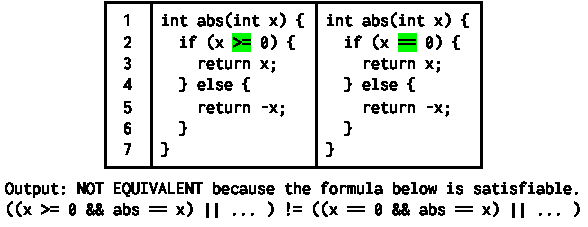
\includegraphics[width=\columnwidth]{code-example.drawio}
      \end{center}
      \vspace{-20pt}

      We hypothesize that developers' understanding of program changes and trust of corresponding tool outputs can be improved if these outputs are enriched with better visualizations and result explanations.
    \end{block}

    \begin{block}{Research Goal}
      Develop an equivalence checking approach that:
      \begin{itemize}
        \item is at least as accurate as existing approaches,
        \item provides more information about behavioral differences,
        \item presents results in a way that is useful for developers,
      \end{itemize}
      thus aiding developer understanding of software changes.
    \end{block}

    \begin{block}{Research Questions}
      \textbf{RQ1}: How can we create an equivalence checking approach that is at least as accurate as existing approaches but provides information about behavioral / semantic differences?
      \vspace{.4ex}

      \textbf{RQ2}: How should we present the collected information (i.e., equivalence checking results, behavioral differences) to developers in order to be most useful for them?
      \vspace{.4ex}

      \textbf{RQ3}: To which degree does the provided information improve (or hinder) the speed, reliability, etc. with which developers are able to reason about software changes?
    \end{block}

    \begin{block}{Research Approach}
      We split our research work into five work packages (WP1–WP5) that produce a total of six research contributions (C1-C6):

      \begin{center}
        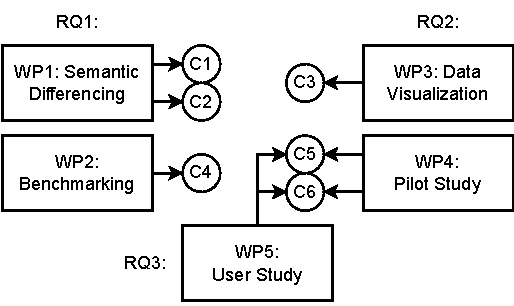
\includegraphics[width=0.8\columnwidth]{research-approach.drawio}
      \end{center}

      WP1 concerns the development of the semantic differencing approach and its prototypical implementation. WP2 evaluates the prototype's accuracy and runtime performance. In WP3, an IDE plugin is created that visualizes the semantic differencing data via source code editor augmentations. WP4 and W5 evaluate the usefulness of the IDE plugin via experiments with developers.
    \end{block}
  \end{column} % End of the first column

  \begin{column}{.02\textwidth}\end{column} % Empty spacer column
   
  \begin{column}{.47\textwidth} % The second column
    \vspace{\shrink}
    \begin{block}{Expected Contributions}
      \begin{itemize}
        \item[\textbf{C1}] An \textbf{approach} for equivalence checking of software programs that provides more information about behavioral / semantic differences than existing approaches.
        \item[\textbf{C2}] An open source \textbf{prototype} that implements the computation of the raw semantic differencing data as a Java application.
        \item[\textbf{C3}] An open source \textbf{prototype} that implements the processing and visualization of the semantic differencing data as an IDE plugin.
        \item[\textbf{C4}] \textbf{Benchmarking results} that compare the equivalence checking accuracy and runtime requirements of our approach to state-of-the-art equivalence checking approaches.
        \item[\textbf{C5}] \textbf{Experimental results} that compare how quickly and accurately developers are able to complete change understanding tasks when using our IDE plugin prototype vs.\ state-of-the-art tools.
        \item[\textbf{C6}] \textbf{Developer feedback} that compares the perceived usefulness of our IDE plugin prototype to state-of-the-art tools.
      \end{itemize}
    \end{block}

    \begin{block}{Preliminary Results}
      For WP1 and WP2, we developed an equivalence checking / semantic differencing tool called PASDA \cite{glock2024pasda} and compared it to the three existing tools ARDiff \cite{badihi2020ardiff}, DSE \cite{person2008dse}, and PRV \cite{boehme2013prv} using the ARDiff benchmark.  PASDA \textbf{correctly classifies} 104 of 141 (\textbf{74\%}) cases, i.e., 9--51 more cases than the three existing tools.

      \vspace{-6pt}
      \begin{center}
        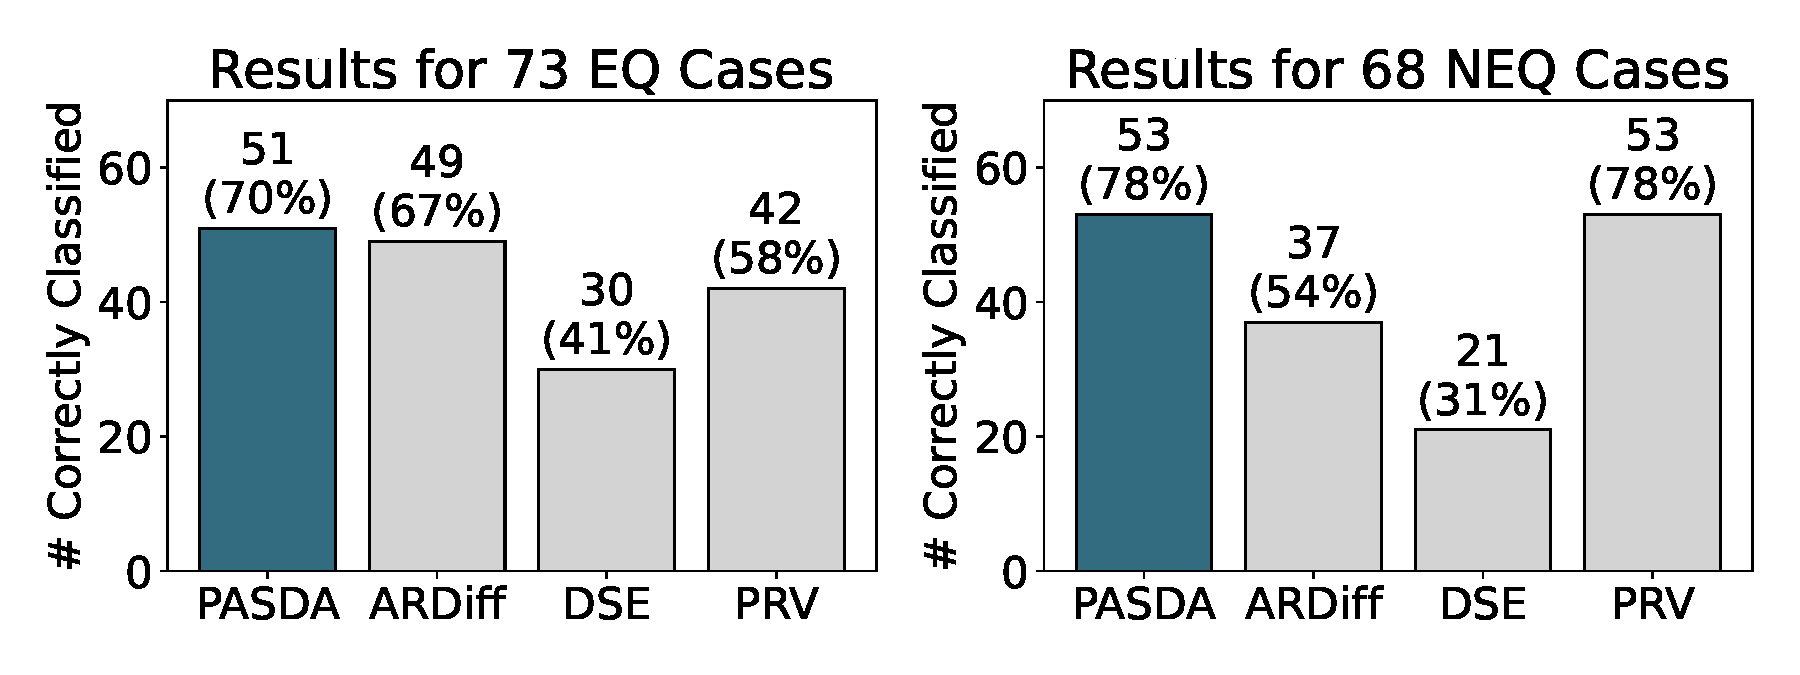
\includegraphics[width=\columnwidth]{classification-accuracy}
      \end{center}
      \vspace{-24pt}

      In addition, for each input partition that PASDA identifies, it aims to provide (i) a \textbf{partition-level non-/equivalence proof}, (ii) concrete and symbolic input and output values, and (iii) the lines of code that are covered by the corresponding execution path. For the two versions of the \texttt{abs} function shown before, PASDA reports:

      \vspace{20pt}
      \begin{table}[]
        \setlength{\tabcolsep}{1ex}
        \begin{tabular}{lrrrrrrr} \toprule
          Input           & \multicolumn{2}{r}{Output} & \multicolumn{2}{r}{Example}                      & \multicolumn{2}{r}{Covered Lines} & Equiv. \\ \cmidrule(l{10pt}r{10pt}){2-3} \cmidrule(l{10pt}r{10pt}){4-5} \cmidrule(l{10pt}r{10pt}){6-7}
          Partition                  & v1     & v2                & v1                     & v2                      & v1            & v2      & Class.               \\ \midrule
          x = 0               &  x     &  x                &  1 \textrightarrow{} 1 &  1 \textrightarrow{}  1 & 1, 2, 3       & 1, 2, 3 & EQ             \\
          x \textgreater{} 0  &  x     & -x                &  1 \textrightarrow{} 1 &  1 \textrightarrow{} -1 & 1, 2, 3       & 1, 2, 5 & NEQ            \\
          x \textless{} 0     & -x     & -x                & -1 \textrightarrow{} 1 & -1 \textrightarrow{}  1 & 1, 2, 5       & 1, 2, 5 & EQ            \\ \bottomrule
        \end{tabular}
      \end{table}
      \vspace{20pt}

      For programs and partitions for which non-/equivalence cannot be proven, PASDA reports a \textbf{best-effort equivalence classification} of MAYBE\_EQ / MAYBE\_NEQ if at least a partial non-/equivalence proof can be provided. Existing tools simply classify such cases as UNKNOWN and provide no further information for them.
    \end{block}

    \begin{block}{References}
      \nocite{*} % Insert publications even if they are not cited in the poster
      \linespread{0.928}\selectfont
      \footnotesize{\bibliographystyle{unsrt}
      \bibliography{references}}
    \end{block}
  \end{column} % End of the second column

  \begin{column}{.02\textwidth}\end{column} % Empty spacer column

\end{columns} % End of all the columns in the poster

\end{frame} % End of the enclosing frame

\end{document}
